\documentclass[english]{article}

\usepackage{graphicx}
\usepackage{grffile}
\usepackage{babel,blindtext}
\usepackage{parskip}
\textwidth = 426pt
\oddsidemargin = 17pt


\title{COS301 : Software Requirements Specification\\
	for The Smart Business Card\\
	}
\date{\today}
\graphicspath{{Pictures/}}

\begin{document}
	\maketitle
	\begin{figure}[!t]
		
\includegraphics{up_logo.png}
	\end{figure}
	\begin{minipage}{0.4\textwidth}
		\begin{flushleft} \large
			\textbf{NAMES:}\\[0.4cm]
			Xolo K Dandashe\\
			Phuti K Setoaba\\
			Thabo Ntsoane\\
			Mpho Mashaba\\	
			Musa Mathe\\
			Khodani M Mufamadi

		\end{flushleft}
	\end{minipage}
	\begin{minipage}{0.4\textwidth}
		\begin{flushright} \large
			\textbf{STUDENT NUMBER:} \\[0.4cm]
		 	14245681\\ 	
		 	13032616\\		
		 	15107532\\	
		 	14309999\\		
		 	15048030\\	
		 	14197520
		\end{flushright}
	\end{minipage}


	
	\pagenumbering{gobble}
	\newpage

	\tableofcontents
	\newpage

	\pagenumbering{arabic}
	

	\section{Introduction}
			

		\subsection{Purpose}
			The purpose of this document is to outline the requirements and design specifications of the SmartCard system. This document provides a detailed explanation of system constraints, interfaces and interactions with other external applications. This document serves as a reference for developing the first version of the system for the development team and will also provide a detailed description of the system for clients and any other interested party.


		\subsection{Scope}
The SmartCard system is a mobile-based application that is used to transfer business data from one device to another using either NFC or QR code scanner. A virtual business card will be generated for the user using the information the user signed up with and will then be transmitted with a single tap using the NFC too available on their smart device. Alternatively the smart device’s camera will be used to scan the QR code on another device. The application should be free to download from either a mobile phone application store or similar services. 


		\subsection{Definition, Acronyms, and Abbreviations}
				This section of the SRS contains definitions, acronyms and abbreviations for the terminology used to describe our system throughout this document.
				\\
				\\
				\begin{tabular}{ |p{3cm}|p{9cm}|  }
				\hline
				\textbf{Term} & \textbf{Definition}\\
				\hline
				User & An actor that interacts with the social media platform\\
				\hline
				Administrator & An actor that is given specific permission for managing and controlling the system\\
				\hline
				QR code & Trademark a type of bar code that can be read both horizontally and vertically, allowing large amounts of information to be encoded in it.\\
				\hline
				NFC & Near field communication \\
				\hline
				\end{tabular}


		\subsection{References}
\begin{itemize}
			\item [[1]] IEEE Software Engineering Standards Committee, "IEEE Std 830-1998, IEEE Recommended Practice for Software Requirements Specifications", October 20,1998 \\
			\item [[2]] QR code. (n.d.). Collins English Dictionary - Complete \& Unabridged 10th Edition. Retrieved April 6, 2018 from Dictionary.com website http://www.dictionary.com/browse/qr-code
		
		\end{itemize}
		\subsection{Overview}
				This SRS  describes the SmartCard System and it is divided into three major sections. \\ 
		
				\begin{tabular}{ |p{3cm}||p{11cm}|  }
				\hline
					Section 1 &  This section details the purpose and scope of the SmartCard system. Definitions, acronyms and abbreviations are listed here to help interpret the SRS appropriately. A list of references to any material that is used in the SRS is included in this section. 
					\\
				\hline
					Section 2 & This section provides the overview of the SmartCard system as a product and describes its context, relations and interfaces to other components of the total system. A summary of functions, general characteristics of the users and any restrictions or contradictions are also outlined in this section. Furthermore any assumptions and dependencies made about the system are also discussed.\\
					\hline
					Section 3 & This section provides a detailed description for each of the system interfaces, hardware interfaces, software interfaces and communications interface. A detailed description of the functionality of each of the functional requirements, performance related capabilities, restrictions and all quality related requirements are included in this section.\\
\hline
				\end{tabular}
	\newpage
	\section{Overall Description}
		
		\subsection{Product Perspective}
			

\subsubsection{User Interfaces}
				
\begin{figure}[!htb]
\minipage{0.32\textwidth}
  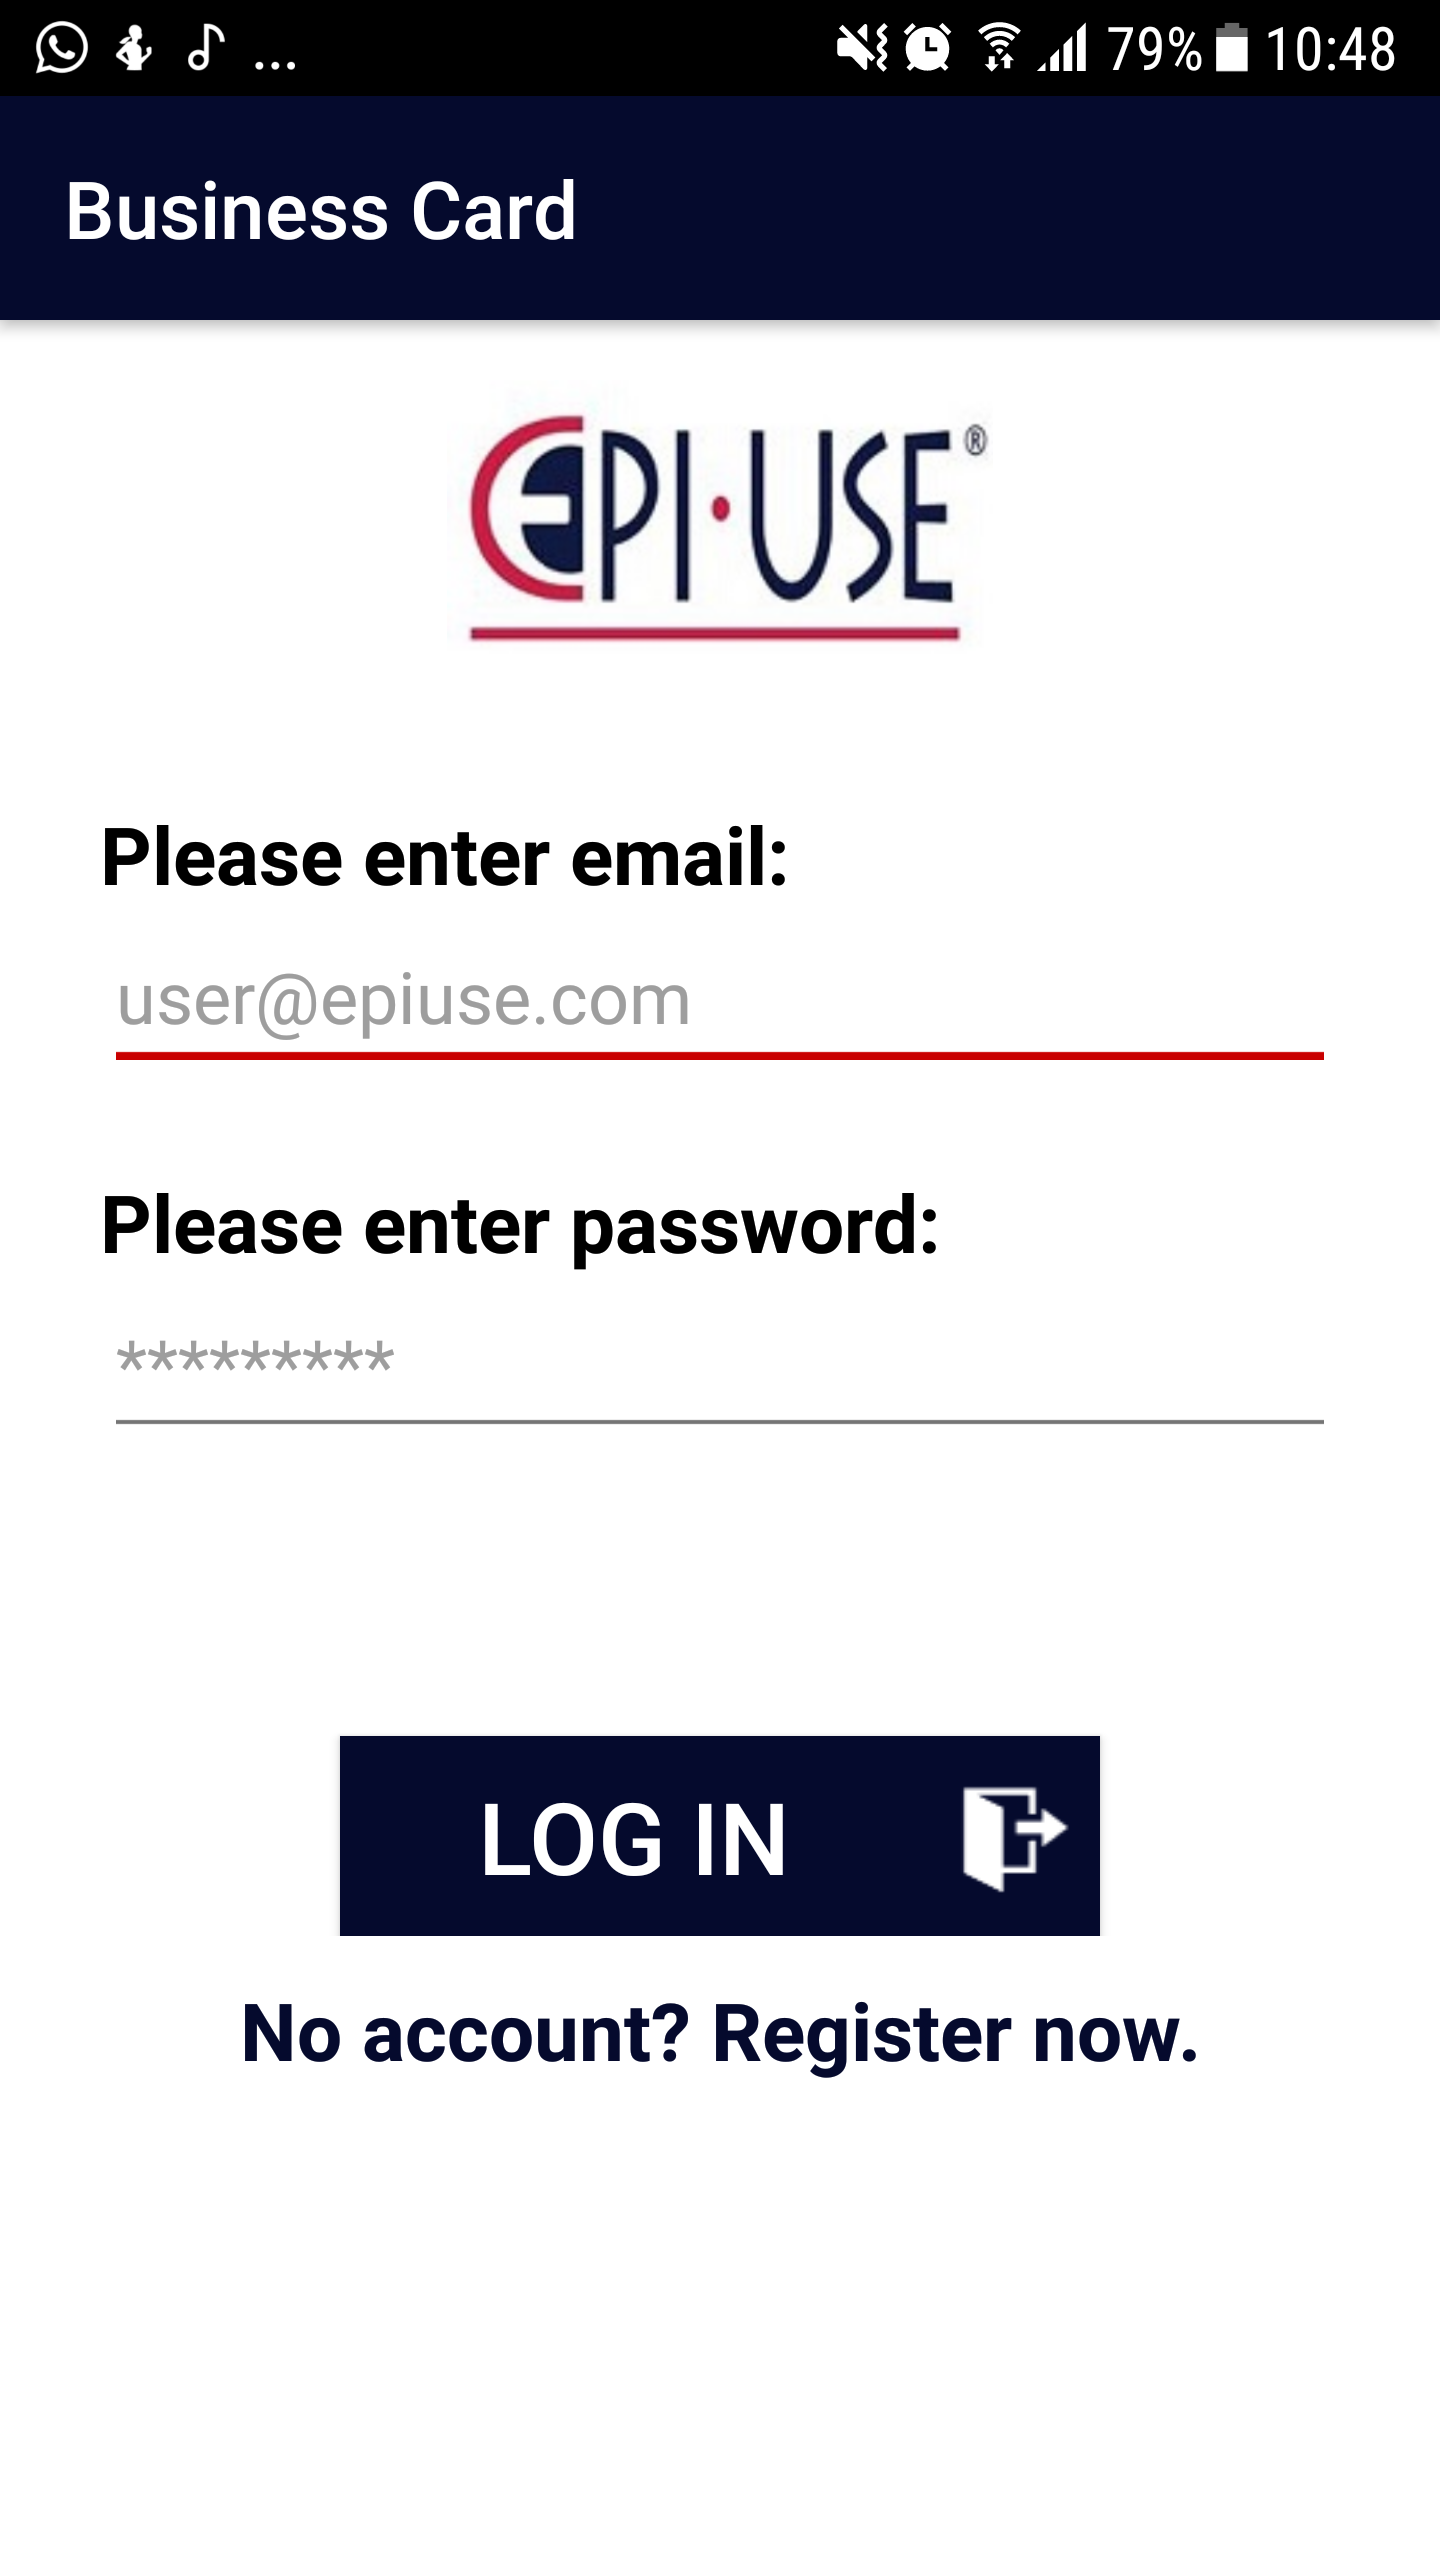
\includegraphics[width=\linewidth]{Login.png}
  \caption{Login}\label{Login}
\endminipage\hfill
\minipage{0.32\textwidth}
  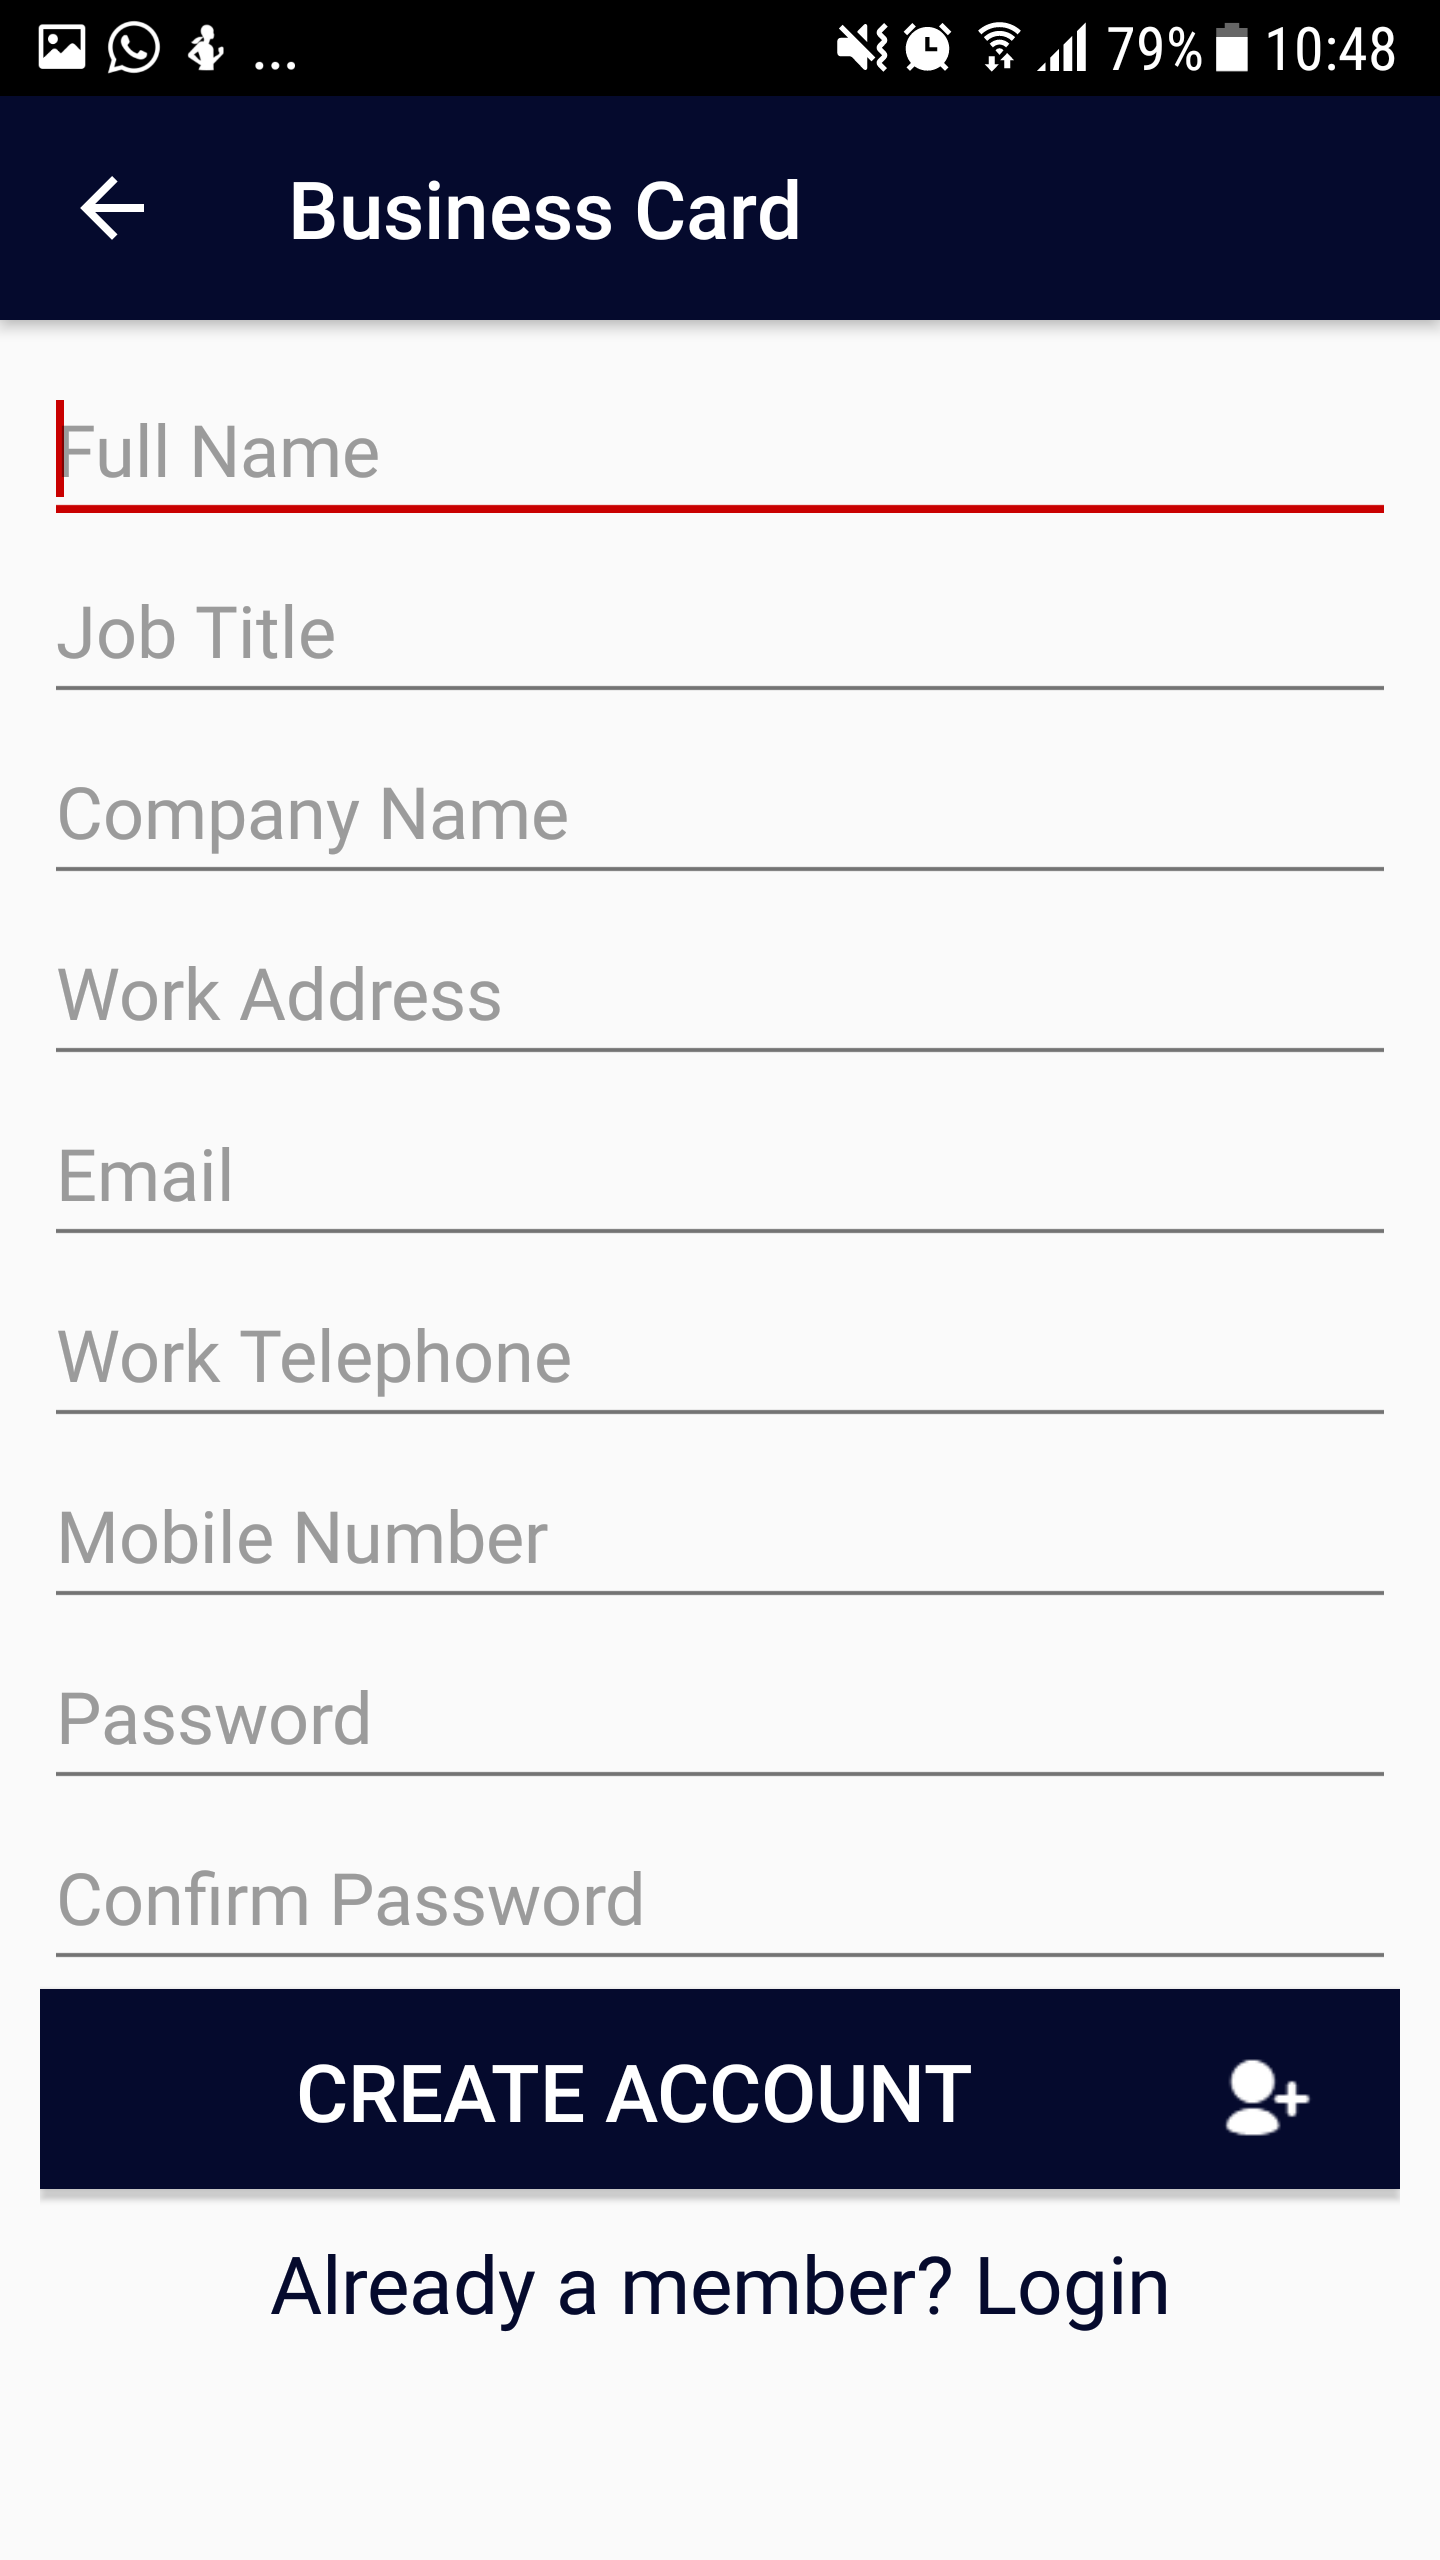
\includegraphics[width=\linewidth]{Register.png}
  \caption{Register}\label{Register}
\endminipage\hfill
\minipage{0.32\textwidth}%
  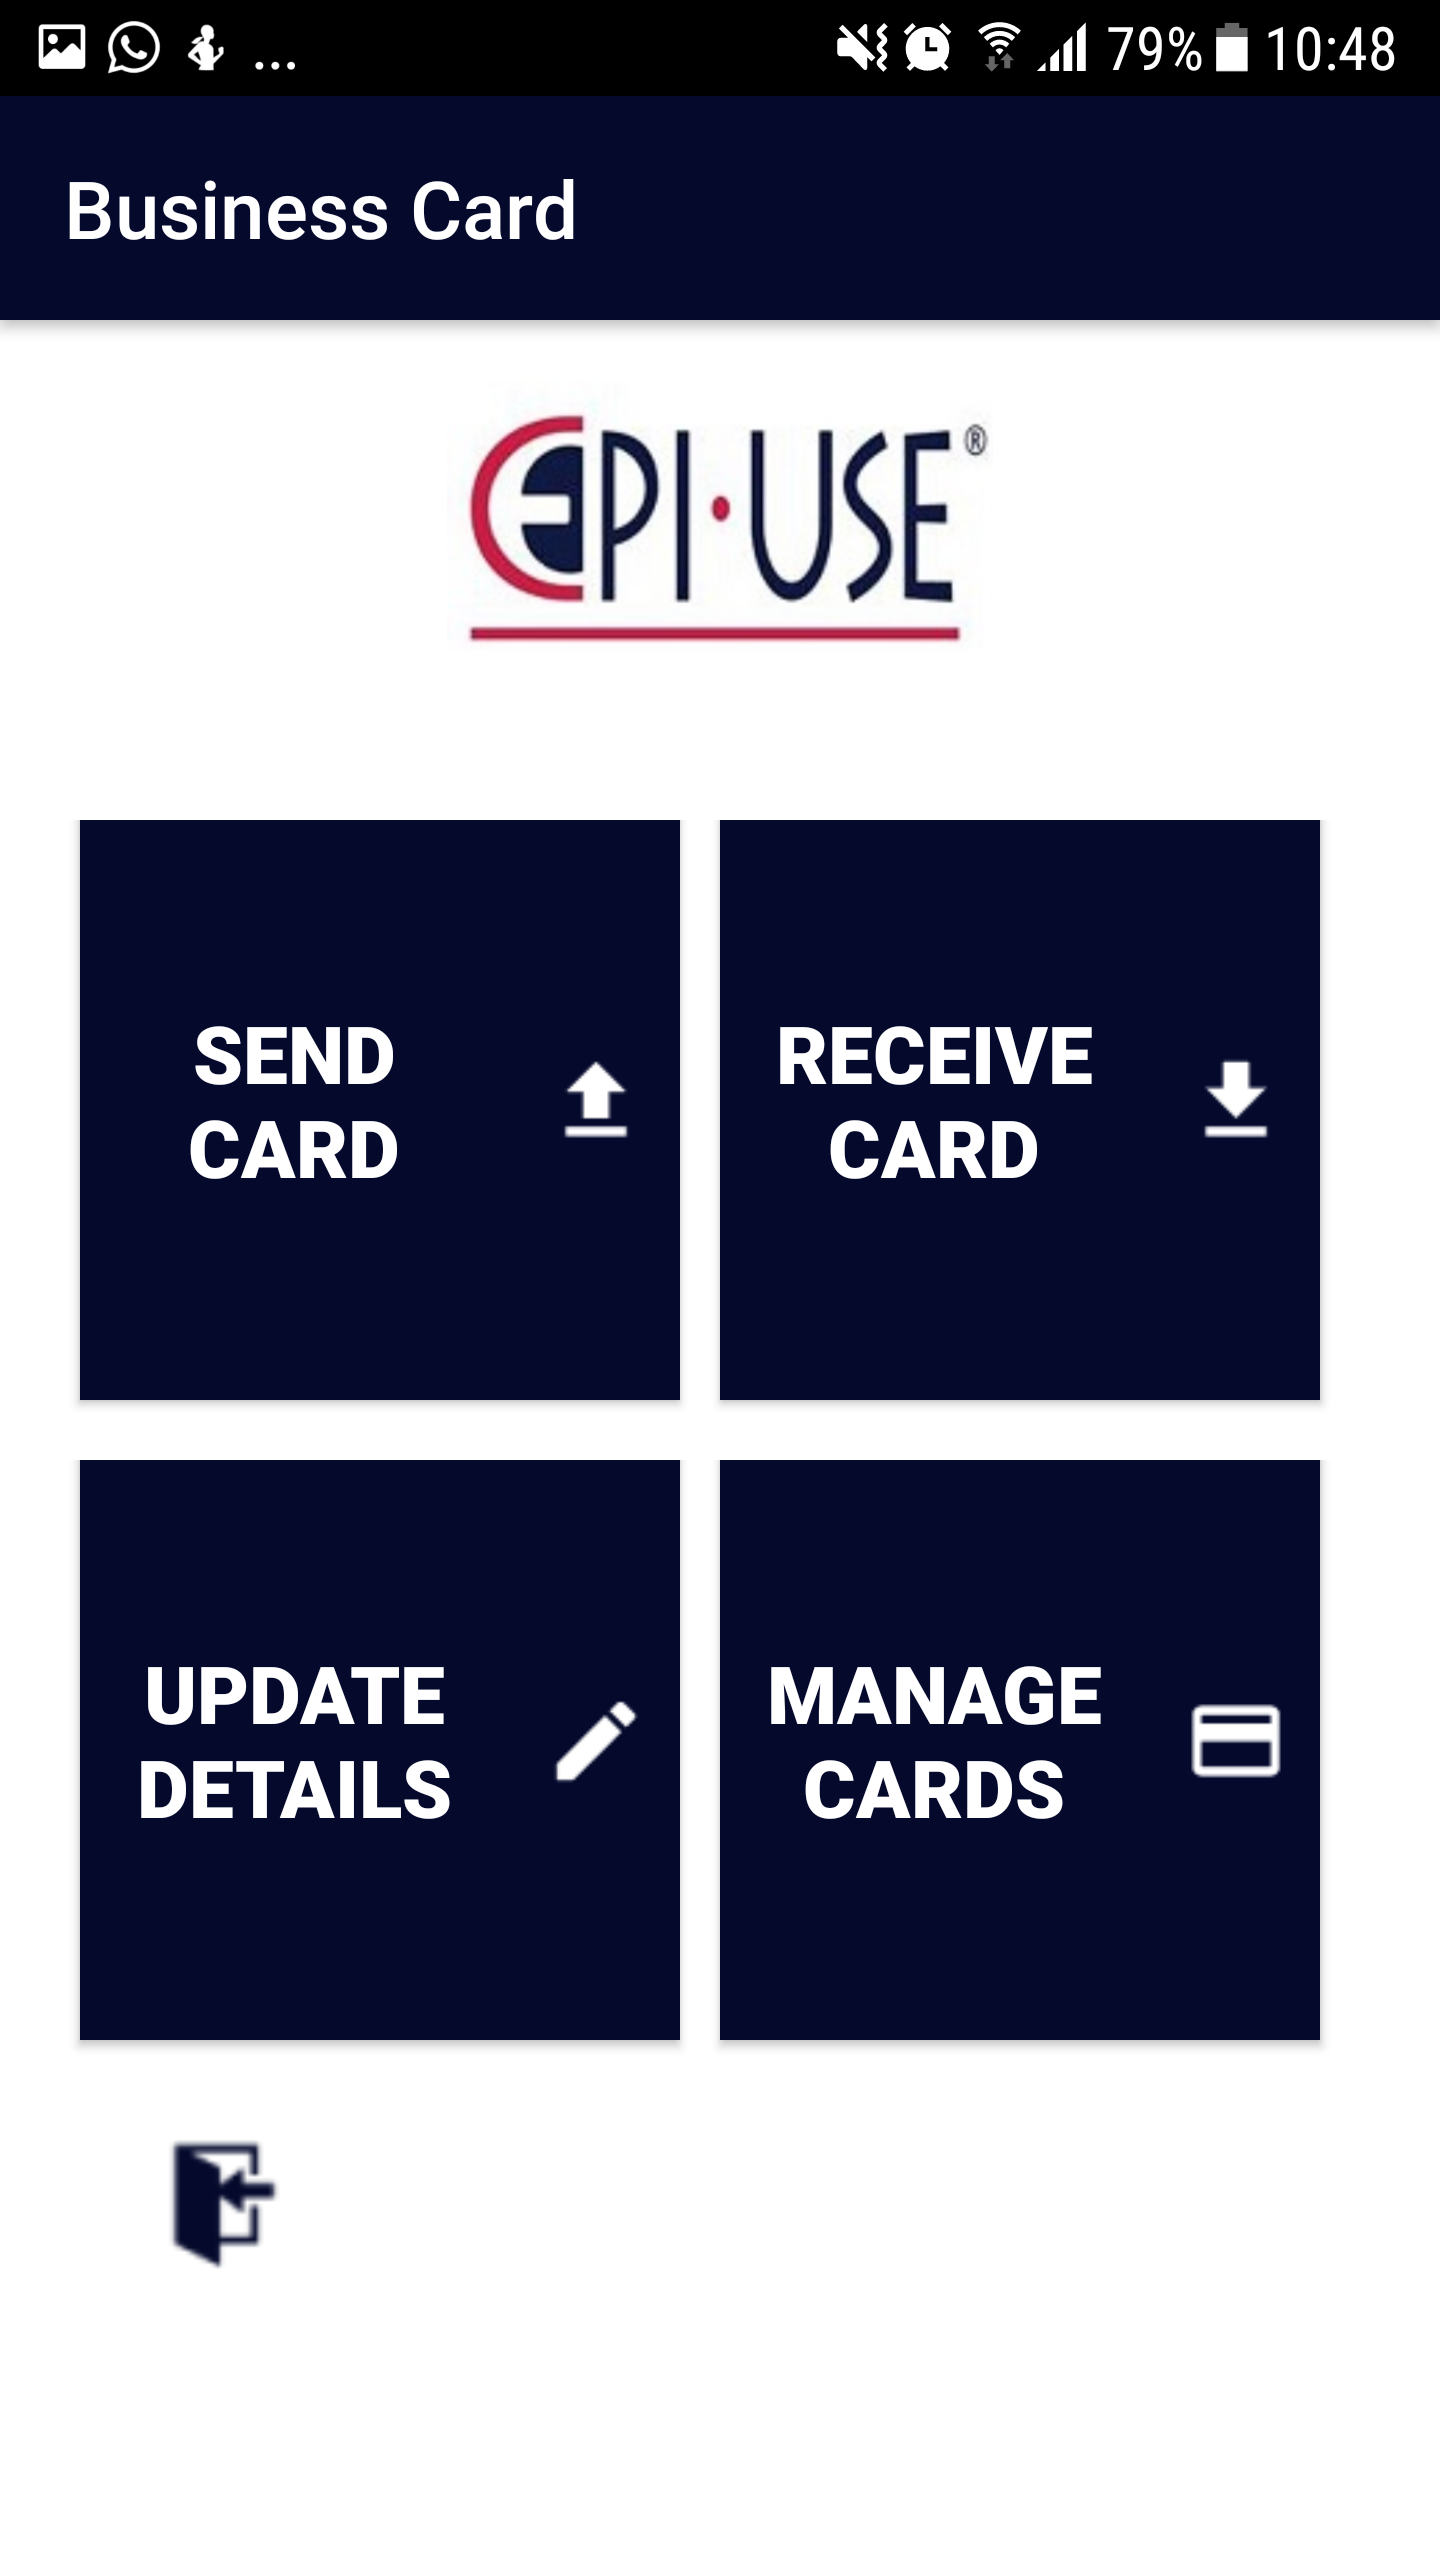
\includegraphics[width=\linewidth]{Main.png}
  \caption{Main}\label{Main}
\endminipage
\end{figure}

								
$\bullet$\ When a user opens the application he/she will see the login page as displayed in figure 1.\\ \\$\bullet$\ If it is a new user then he/she will click on the register link which will then take the user to the register form as shown in figure 2.\\ \\$\bullet$\ After the user successfully registers then the user will be able to see the main page as displayed by figure 3.\\ \\$\bullet$\ The main page shows that the user can be able to send a business card to another user, the user can also receive business cards from other users, the user can update his/her details on the application and also manage the cards which have been received/read from other user.


		\subsubsection{System Interfaces}


$\bullet$\ Users use mobile device to read/write to business card using the application.\\
\\$\bullet$\ The application stores and retrieves information from database.\\
\\$\bullet$\ The web portal reads/writes to the business cards then stores the information to the database.\\
\\$\bullet$\ The mobile application will integrate google maps to it so that people can use it for location purposes when searching for another user’s work area.

\begin{figure}[ht!]
\centering
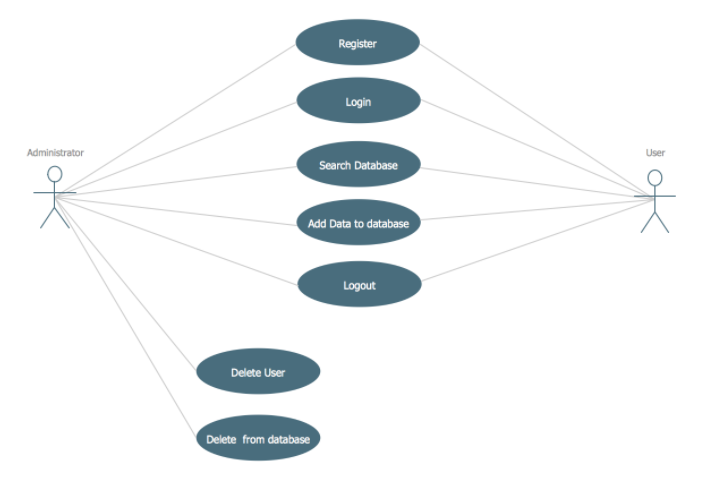
\includegraphics[width=90mm]{system.png}
\caption{Block diagram for the system }
\end{figure}	
						

\subsubsection{Hardware Interfaces}				
$\bullet$\ Devices with NFC will be using the chip on their phones to read from the NFC business card.\\ \\$\bullet$\
The devices which do not have the NFC chip will be using the QR code on the business card to scan the information to the phone.\\ \\$\bullet$\
The web portal will be accessed using a laptop or computer.\\ \\$\bullet$\
The NFC device will be used to read/write to NFC business card.(Check diagram below)\\
\begin{figure}[ht!]
\centering
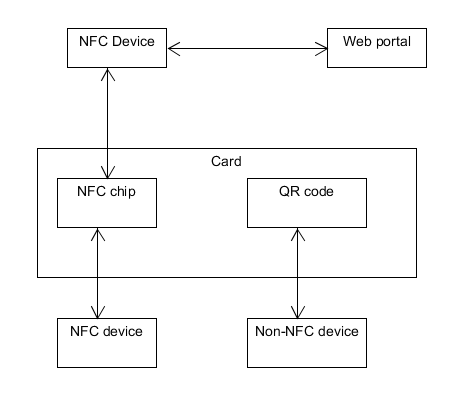
\includegraphics[width=60mm]{Hardware.png}
\caption{Hardware interface block diagram }
\end{figure}

				   
\subsubsection{Software Interfaces}

\begin{tabular}{ |p{3cm}|p{9cm}|  }
				\hline
				\textbf{} & \textbf{Definition}\\
				\hline
				Cards & Will have both QR and NFC chips embedded on them.\\
				\hline
				Application & Android studios
$\bullet$\ Java
$\bullet$\ Barcode API
$\bullet$\ NFC API
\\
				\hline
				 Web portal & HTML5,CSS,PHP,Javascript\\
				
				\hline
				 Google maps & Google maps API\\
				\hline
				 Database & Firebase database–JSON\\
				\hline
				
				\end{tabular}
\begin{figure}[ht!]
\centering
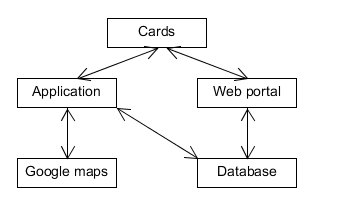
\includegraphics[width=60mm]{Software.png}
\caption{Software interface block diagram}
\end{figure}
			
					
\subsubsection{Communications Interfaces}

\begin{figure}[ht!]
\centering
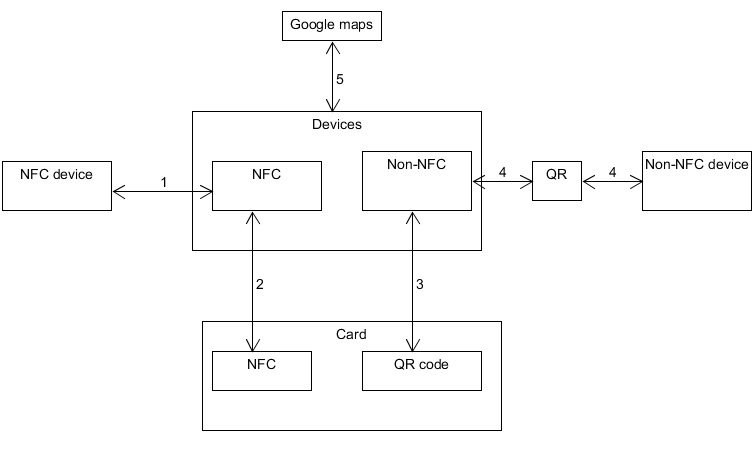
\includegraphics[width=90mm]{communication.png}
\caption{Communication block diagram }
\end{figure}

				1.	NFC Device to NFC device communication\\
$\bullet$\ A phone with an NFC chip exchanging information with another phone having an NFC chip.\\
2.	NFC Device to a NFC business card chip communication\\
$\bullet$\ A phone with NFC chip reading/writing to a NFC business card.\\ 
3.	Device to QR card communication\\
$\bullet$\ A phone without NFC reading business card which has both NFC chip and QR reader.\\
4.	Device to device communication\\
$\bullet$\ Phone without NFC generating QR code to be read by another phone without NFC.\\
5.	Device connecting to Google maps\\
$\bullet$\ Mobile app communicates with the google maps to get the get the office location of another user.(Check diagram above)


			
				
						\subsubsection{Operations}


\begin{figure}[ht!]
\centering
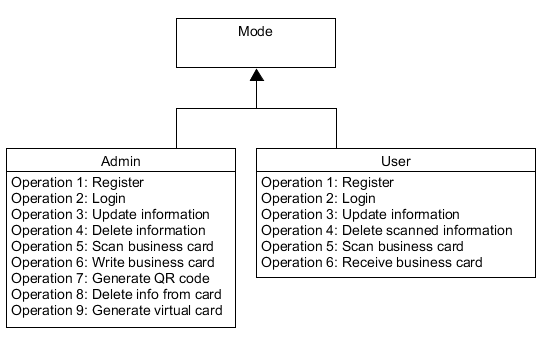
\includegraphics[width=90mm]{operation2.png}
\caption{User mode operations }
\end{figure}				



\begin{figure}[ht!]
\centering
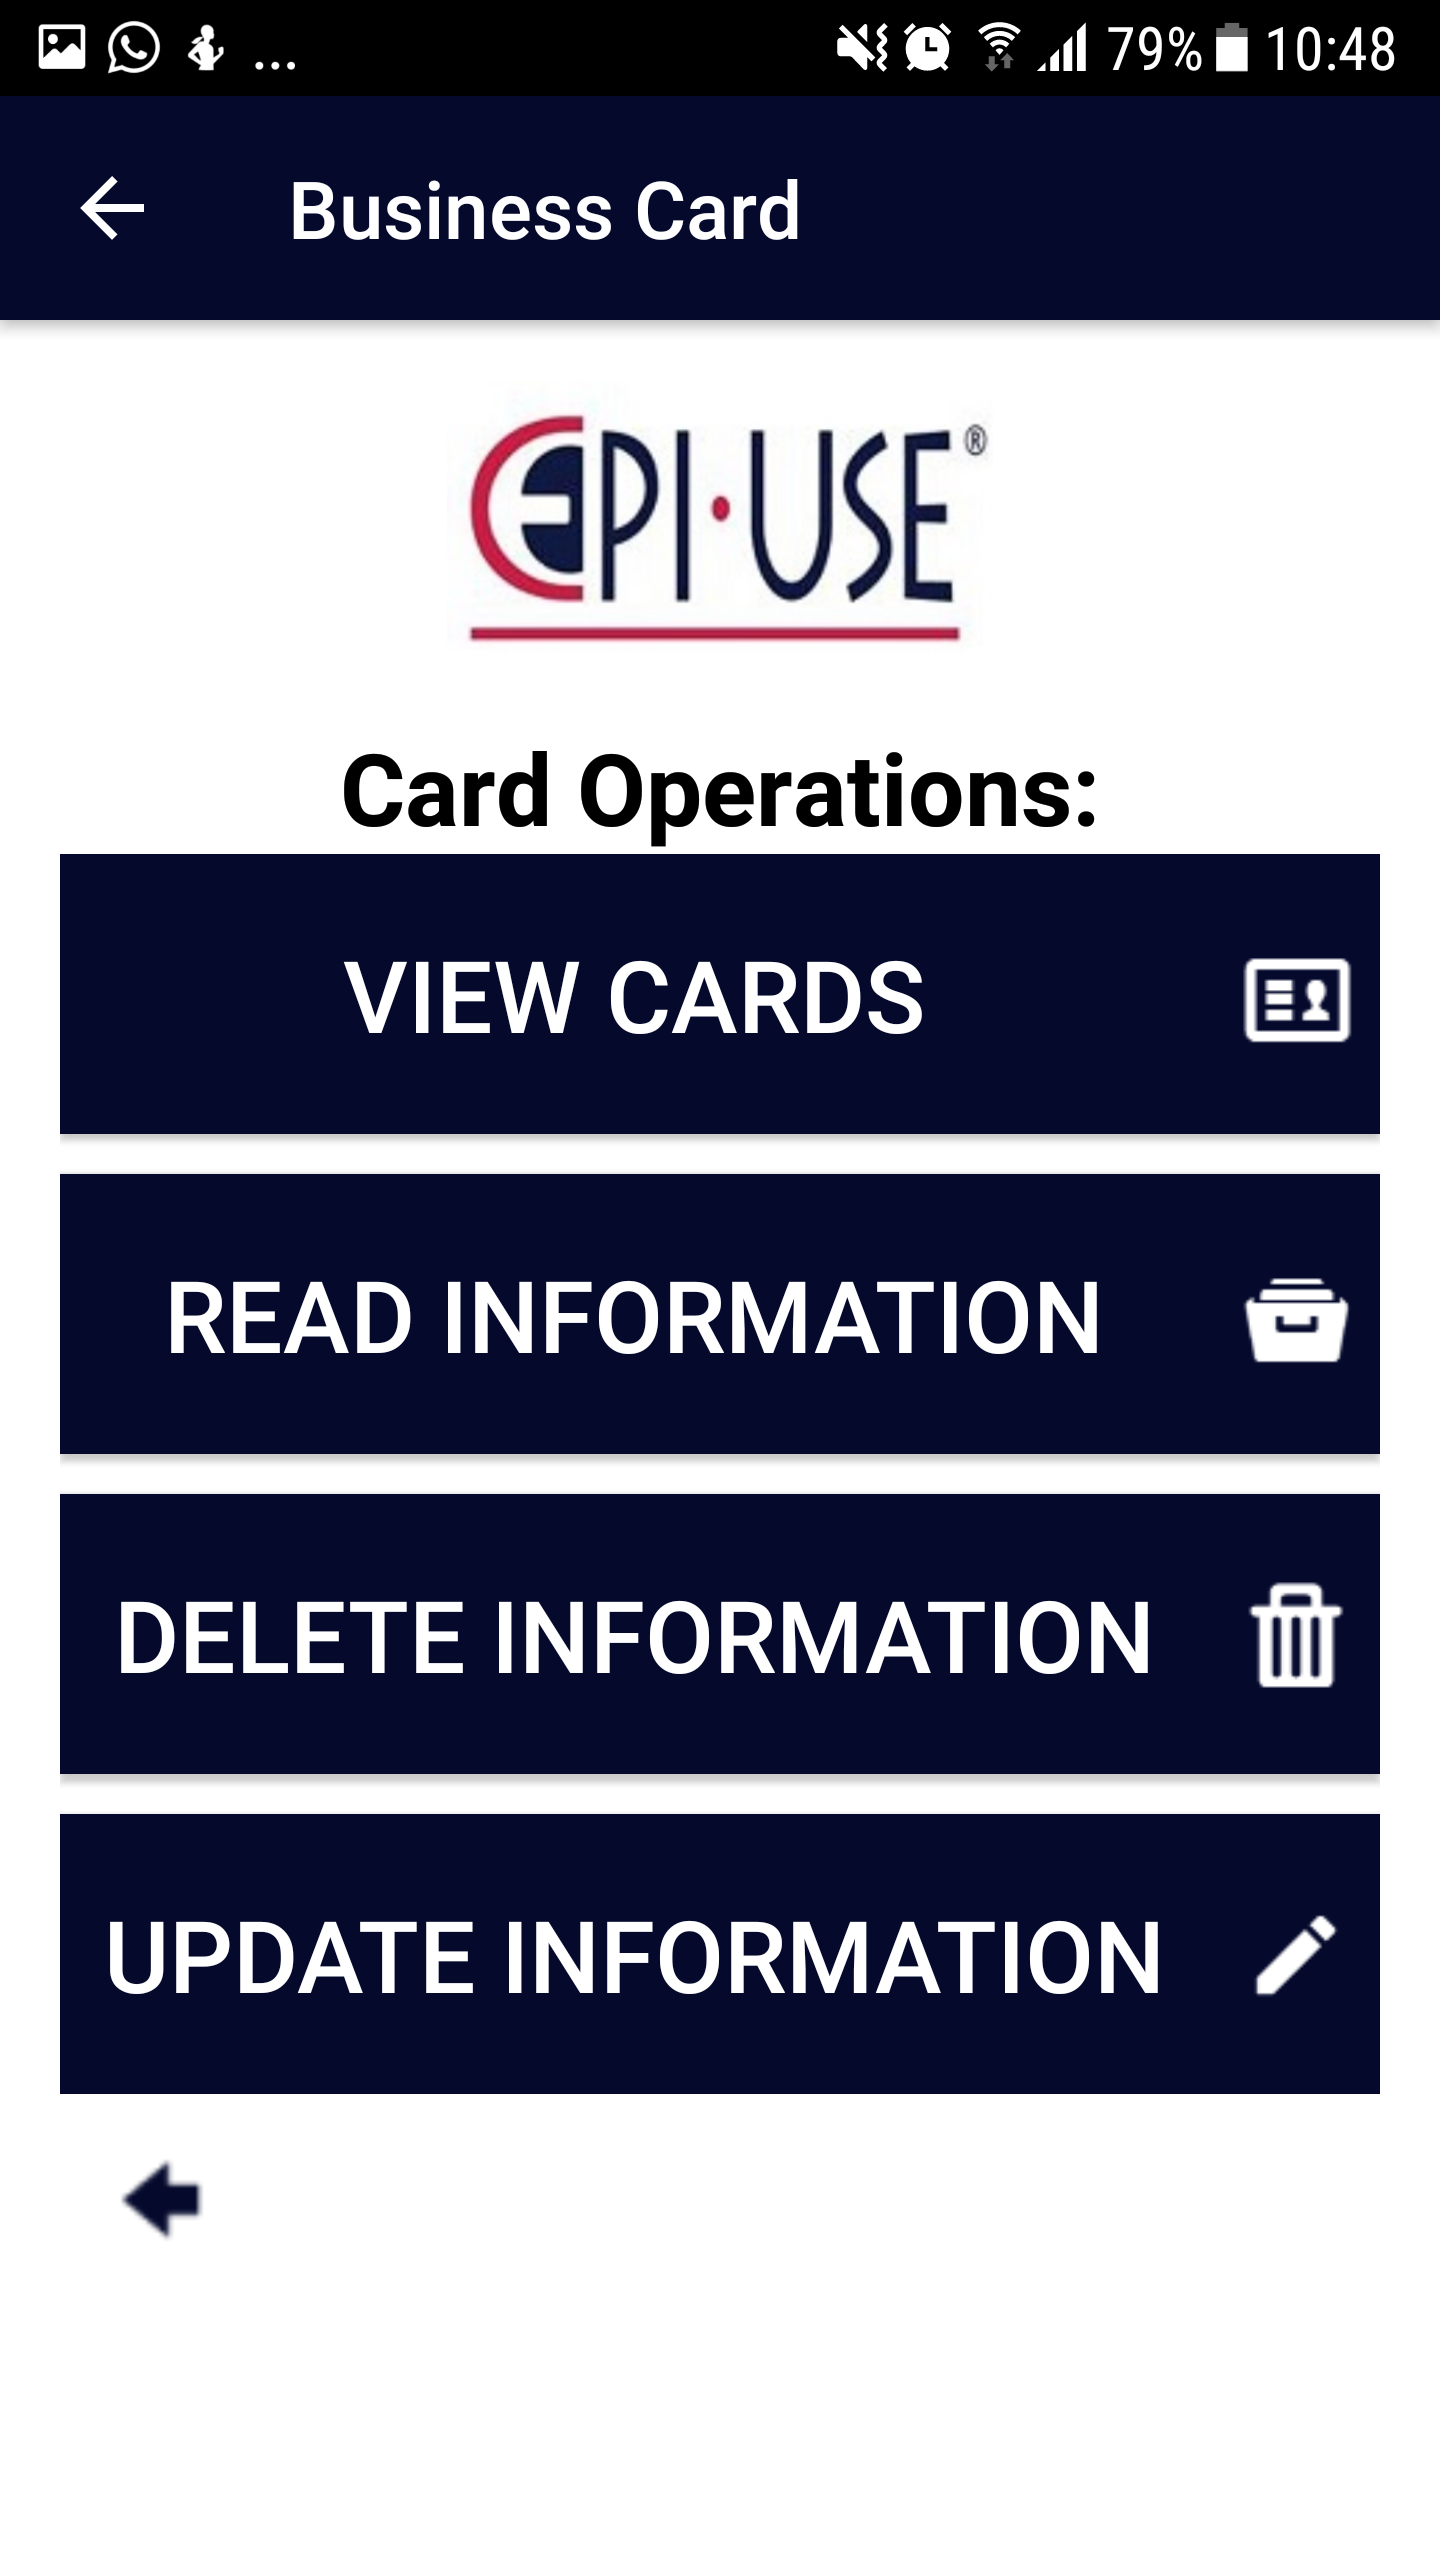
\includegraphics[width=30mm]{operations.png}
\caption{Card Operations }
\end{figure}


$\bullet$\ View cards– User can view the cards which were scanned.
\\$\bullet$\ Delete information- User can decide to delete the details of the cards which were scanned .
\\$\bullet$\ Update information- User can update the information to the card.





				\subsection{Product Functions}
				\begin{itemize} 
					\item Sign Up
					
					\subitem
					- Every user needs to sign up in order to use the product.
					\item
					Log in
					\subitem
					The user needs to log in using the email and password they used when signing up.
					\subitem 
					Once the user logs out, the user can only use the application if they log back in.
					\item 
					Send Card
					\subitem
					Users are able to send their business cards to other users of the application via QR code or NFC functionality.
					\item
					Receive Card
					\subitem
					Users are able to receive business card information through tapping their mobile device on the 'smart business card', putting phones back to back and receive through NFC functionality or scanning a generated QR code.
					\item 
					Delete Card
					\subitem
					Users are able to delete their business card information.
					\item
					Modify Card
					\subitem
					Users are able to modify their business card information on the chip through the application.
					\item
					Generate QR Code
					\subitem
					For mobile devices without NFC functionality, QR codes can be generated for sending or receiving purposes.
					\item
					Embed QR code to physical code
					\subitem
					The System will generate a QR code that will be on the physical business card.
					\item
					Scan physical Business Card
					\subitem
					The product can scan physical business cards and enable users to save and share the information electronically.
					\item
					Card shelves
					\subitem
					The product allows sorting of different business cards according to different categories.
					
					\item
					Search card
					\subitem
					Product enables users to search saved business cards according to first or last name, Company and position.
					\item
					GPS functionality	
					\subitem
					The product will use Google API's in order to give directions to the specified address mentioned on an individuals business card.
				\end{itemize}

				\subsection{User Characteristics}
				\begin{itemize}
					\item
					Users can be individuals. The product is most likely to be used by:
					\subitem
					- Intern's looking for jobs.
					\subitem
					- Employed workers looking for new positions
					\subitem
					- Companies as a whole
					\subitem
					- Human Resources
					\item 
					The user needs moderate knowledge of:
					\subitem 
					- Using phone applications, 
					\subitem 
					- Computer Security,  
					\item 
					The user must be able to: 
					\subitem
					- Type on a keyboard and navigate through the application
					\subitem
					- Read and Write information, must be literate.
				\end{itemize}
				
			
				\subsection{Constraints}
            
				
				$\bullet$\  The constraints on the project are related to the provision of hardware resources to implement and test. Our project is coded mainly in android studio which may require a lot of time when building. At present we are using laptops                                 				that are only on 2/4 gig RAM running intel inside processor which can be very slow when building a project during testing. For better perfomance and more efficient building, laptops that use atleast 6gig of RAM and a i5 processor would be 							beneficial.\par

                                	$\bullet$\ The mobile devices that are going to run our application are constrained by NFC technology. The phone you're using to run the application needs to have NFC technology on it. To overcome this particular constraint, will make use of QR codes 					as a substitute to mobile devices that do not contain NFC technology on them. 

                                	$\bullet$\ Normal business cards without any NFC chips embedded in them will also be a constraint when using the system. Because these cards don't have NFC chips, we are going to have  to scan them to our sytem and embed a QR code on them so 					they can also be used.

                                	$\bullet$\  Another constraint is that our application will only work on android phones so people that use other operating systems on their mobile devices won't have acces to it.  
				
				\subsubsection{Assumptions and Dependencies}
				
				 $\bullet$\ It assumed that the user is familiar/has basic knowledge with mobile applications  and also familiar with handling the keyboard on the phone for registering and login in operations.

                                 	 $\bullet$\ It is assumed that the user will have mobile data on their phone when using our location service because Google maps will be integrated in our application which requires mobile data/ WI-FI to work.

                                	 $\bullet$\ User Manual will be provided for the application 
		
		\newpage

	\section{Specific Requirements}
				\subsection{External Interface Requirements}
						Since the prototype will  be developed for Android systems and later on expanded to iOS ,this part of the specification will primarily assume the Android OS is the operating system for the system.
						\subsubsection{Interfaces} 
					         The app will require system privileges to make use of certain features and information provided by the Android OS.
						 \begin{itemize}
							      \item \textbf{NFC}\\
					        The system will be dependant on the device's NFC system services to be able to read the nfc smart card and also send                              business cards via NFC to another device.Access to this feature forms the backbone of the app as most of the subsystems are dependant on it.
								\item \textbf{Camera}\\
						If a mobile device does not have a NFC chip our app will use the camera on the phone to scan a QR code .
						\end{itemize}
						\subsubsection{User Interfaces}
						    There will be a unified user interface which can be broken down into 4 subsystems all of which will be displayed 		           simultaneously. The 5th subsystem (Searching) will tie into the navigational subsystem \\
                                                  \begin{itemize}
					        \item \textbf{Send Card}\\
						Users will use the Send Card subsystem to Send thier business card information to another device using NFC or a QR code that has been generated .The user will select the option they want ,if NFC is selected the system will check whether the device has a NFC and if its on after that 	it will attempt to send the business card to a receiver and will display a popup showing whether the transfer was succesfull or not.				       

						\item \textbf{Recieve Card}\\
						Users will use the receive card subsystem to receive a business card from a sender which might be a smartcard or another device either through NFC or scanning the QR code.

						\item \textbf{Update Details}\\
						This will give the user the ability to update all thier information .
						
						\item \textbf{Manage Cards}\\
						Users and Administrators will interact with the update subsystem with the administrators having more privillages.The users will be able to view their saved cards while the admin will be able to view cards ,write ,update and delete information from a smartcard.

                                                 
                                              
                                                \item \textbf{Searching}\\
						This will be a minor add-on to the Manage Cards Subsystem which will allow users to search for business cards they have saved on their device.
                                                  \end{itemize}
                                              \subsubsection{System Interfaces}
							\begin{itemize}
    						    \item \textbf{An android phone } \\
    						    Android devices are the most commonly used devices, so development will initially focus on these devices. There are android devices with many varying specifications, but we will focus on newer models in order to simplify the prototype. \\
    
    						\end{itemize}
                                               \subsubsection{Software Interfaces}
        					\begin{itemize}
        					    \item \textbf{Android NFC API}\\
        					    This would be our tool of choice as it covers the basis for sending and receiving data through NFC ,which our system requires for successful implementation.
						 \item \textbf{Google Maps API}\\
        					    This would be our tool of choice as it covers the basis for navigation which will be an add on at a later stage for our system.
        					    \item \textbf{Other}\\
        					    Other libraries and API's will then be added to the project later to cater for any extensions once our core features have been implemented.
        					\end{itemize}
                                              \subsubsection{Hardware Interfaces}
    						\begin{itemize}
						  \item \textbf{NFC chip} \\
						The nfc chip on the phone and the smartcard are the ones to be used for the transfer of information.
    						    \item \textbf{Camera} \\
    						    We will use the Camera if a phone does not have a NFC chip to read a QR code that consist of the business card information . \\
						\end{itemize}
						\subsubsection{Communication Interfaces}
						\begin{itemize}
    						    
    						    \item \textbf{Near field communication (NFC)} \\
    						    We will make use NFC to write and read data from a NFC smart card.    						    
    						  
    						    \item \textbf{E-mail} \\
    						    We will use email for registration and login, which will then allow us to identify different users.  \\
    						\end{itemize}

 				\subsection{Functional Requirements}
				In the following section, the fundamental functions of the application will be specified.\\
				\textbf{User Class 1- User}\\
				\textbf{Functional Requirement 1.1}\\
				\textbf{ID}:FR1\\
				\textbf{Title}: User Registration\\
				\textbf{Description}: Once the application is on the user's phone, she or he is able to register using their mobile device.\\
				\textbf{Previous requirement needed}: None\\
				
				\textbf{Functional Requirement 1.2}\\
				\textbf{ID}:FR2\\
				\textbf{Title}: Log in\\
				\textbf{Description}: The user should use their creditionals to log into the application, using their email with the corresponding password to successfully enter. If the email or password do not correspond with what was entered, the user will not be allowed to proceed.\\
				\textbf{Previous requirement needed}: FR1\\
				
				
				\textbf{Functional Requirement 1.3}\\
				\textbf{ID}:FR3\\
				\textbf{Title}: Select An Option from Menu\\
				\textbf{Description}: Once logged in, the user will be given a menu in which they can select an option.\\
				\textbf{Previous requirement needed}: FR2\\
				
				\textbf{Functional Requirement 1.4}\\
				\textbf{ID}:FR4\\
				\textbf{Title}: Log out\\
				\textbf{Description}: From the menu, the user will be able to log out of their account and release control over their.\\
				\textbf{Previous requirement needed}: FR3\\
				
				\textbf{Functional Requirement 1.5}\\
				\textbf{ID}:FR5\\
				\textbf{Title}: Receive Card\\
				\textbf{Description}: The user is able to recieve a virtual business card from another device. Although two options to receive a virtual business card are given, the exchange can be by either by scanning a QR Code or Tapping another phone using NFC.\\
				\textbf{Previous requirement needed}: FR3\\
				
				\textbf{Functional Requirement 1.6}\\
				\textbf{ID}:FR6\\
				\textbf{Title}: Scan QR Code\\
				\textbf{Description}: The user will be able to scan another user's QR Code containing their information, then storing it on their device.\\
				\textbf{Previous requirement needed}: FR5\\
				
				\textbf{Functional Requirement 1.7}\\
				\textbf{ID}:FR7\\
				\textbf{Title}: Recieve via NFC\\
				\textbf{Description}: The user will be able to be tapped by another device to exchange information, then storing it on their device. Both devices must have a NFC chip inorder for this requirement to be successful.\\
				\textbf{Previous requirement needed}: FR5\\
				
				\textbf{Functional Requirement 1.8}\\
				\textbf{ID}:FR8\\
				\textbf{Title}: Send Card\\
				\textbf{Description}: The user will be able send their virtual business card. They will have an option to either generate a QR code that will scanned or a virtual business card via NFC, containing their information.\\
				\textbf{Previous requirement needed}: FR3\\
				
				\textbf{Functional Requirement 1.9}\\
				\textbf{ID}:FR9\\
				\textbf{Title}: Generate QR Code\\
				\textbf{Description}: The user will be able to generate a QR Code containing their information. The QR Code will may be scanned by a recieving user.\\
				\textbf{Previous requirement needed}: FR8\\
				
				\textbf{Functional Requirement 1.10}\\
				\textbf{ID}:FR10\\
				\textbf{Title}: Send via NFC\\
				\textbf{Description}: The user will be able to tap another device to exchange information. Both devices must have a NFC chip inorder for this requirement to be successful.\\
				\textbf{Previous requirement needed}: FR8\\
				
				\textbf{Functional Requirement 1.11}\\
				\textbf{ID}:FR11\\
				\textbf{Title}: View Details\\
				\textbf{Description}: The user will be able to view their current details and decide whether they want to update them.\\
				\textbf{Previous requirement needed}: FR3\\
				
				\textbf{Functional Requirement 1.12}\\
				\textbf{ID}:FR12\\
				\textbf{Title}: Update Details\\
				\textbf{Description}: The user's will be able to update their details.\\
				\textbf{Previous requirement needed}: FR11\\
				
				\textbf{Functional Requirement 1.13}\\
				\textbf{ID}:FR13\\
				\textbf{Title}: Select Option from Card Management\\
				\textbf{Description}: The user will be able to select which option they want.\\
				\textbf{Previous requirement needed}: FR3\\
				
				\textbf{Functional Requirement 1.14}\\
				\textbf{ID}:FR14\\
				\textbf{Title}: View Business Cards\\
				\textbf{Description}: The user will be able to see what previous cards they have stored and access the details of each card.\\
				\textbf{Previous requirement needed}: FR13\\
				\subsection{Performance Requirements}
				In the following section, the performance expectations and measurements of the application will be specified.
				
				\textbf{Quality Requirement 1}\\
				\textbf{Title}: Usage of search feature\\
				\textbf{Description}: The user must easily understand how to use the search feature. The user must be able to use keywords to find specific business cards.\\
				
				\textbf{Quality Requirement 2}\\
				\textbf{Title}: Results of search feature\\
				\textbf{Description}: The user must get a result set with every search in a list format which the user can understand and use accordingly, unless the result set is empty which means a notification of an empty result set was found.\\
				
				\textbf{Quality Requirement 3}\\
				\textbf{Title}: Usage of Location services\\
				\textbf{Description}: Location services provided by the user's device should give an almost accurate location, that the user should be able to understand which will be used to save the user's address when registering.\\
				
				\textbf{Quality Requirement 3}\\
				\textbf{Title}: Usage of Navigation services\\
				\textbf{Description}: Navigation services provided by the user's device should give an almost accurate path,that the user should be able to understand which will be followed by the user to the specified address.\\
				
				\textbf{Quality Requirement 4}\\
				\textbf{Title}: Usage of QR code\\
				\textbf{Description}: Information should not be lost or modified during conversion of information from the virtual business card to a QR code.\\
				
				\textbf{Quality Requirement 5}\\
				\textbf{Title}: Usage of QR code\\
				\textbf{Description}: Information should not be lost or modified during conversion into from a QR code to a virtual business card.\\
				
				\textbf{Response Time}
				\textbf{Quality Requirement 6}\\
				\textbf{Title}: Response of a search\\
				\textbf{Description}: The response time of a search initiated by a user to look for a specific business card.\\
				\textbf{Meter}:Measurements obtained from 10 Business card searches during testing.\\
				\textbf{Must}:\\
				\textbf{Wish}:\\
				
				\textbf{Quality Requirement 7}\\
				\textbf{Title}: NFC Exchange\\
				\textbf{Description}: Exchanging information between two devices via NFC.\\
				\textbf{Meter}:Measurements obtained from 10 NFC Exchanges during testing.\\
				\textbf{Must}:\\
				\textbf{Wish}:\\
				
				\textbf{Quality Requirement 8}\\
				\textbf{Title}: QR Exchange\\
				\textbf{Description}: Exchanging information between two devices via QR.\\
				\textbf{Meter}:Measurements obtained from 10 QR Exchanges during testing.\\
				\textbf{Must}:\\
				\textbf{Wish}:\\
				The application must:
				\begin{itemize}
					\item 
					Check if NFC chip is available in the device before exchanging information to and from another device.
					\item
					Check if Camera is available in the device for before QR scanning.  
					\item
					Display a message if an error has occurred.
					\item
					Ensure QR scan should be successful within 5 seconds after acquiring the QR code.
					\item
					Ensure NFC exchange should be completed within 2 seconds.
					\item
					Exchange information between two user only.
					\item
					Be able to manage a large sum of small sized virtual business cards. Many objects of a small size.
					\item
					Be able to deal with fault tolerance by having down-time of at least 7\% of the time. 
				\end{itemize}
				\subsection{Design Constraints}
				\paragraph\indent
				This application is constrained in two main areas, namely hardware and software. We will look at these two areas separately.
				 \subsubsection{Hardware}
				
						$\bullet$\ The SmartCard can only store a small amount of information since it has limited space.

						$\bullet$\  NFC has a small range so the phone and card or phone and phone need to be in contact.
					
				
				 \subsubsection{Software}
					
					$\bullet$\ The system must be able to operate efficiently.

					$\bullet$\ The system should securely transfer information.

                                                     $\bullet$\  The system must be able to keep all user information secure.
					
				 \subsubsection{Other}
				
					
									\newpage
				\subsection{Software System attributes}
				
				\subsubsection{Reliability}
    				The system must be able to perform all its functions under the stated conditions and produce correct and consistent results. 
    				
				
				\subsubsection{Security}
    					\begin{itemize}
					\item Only administrators must be able to write information to the SmartCard.
					\item All data must be transmitted in a securely.

					\end{itemize}
    				
				\subsubsection{Manageability}
					\begin{itemize}
							\item We will make use of open-source libraries to ensure that there is less code to maintain.
							\item The system should be developed in a manner that will allow developers to extend features with ease.
						\end{itemize}
	
				    
				\subsubsection{Efficiency}
				  The system must be able to perform various functions and produce desired results with minimum expenditure of time and resources.which is the sending of correct business card information and also store the correct information on the receiving device.
				\subsubsection{Availability}
	                          The system must be always available provided that the minimum hardware requirements are met.
				 
	
				
				

				\subsection{Other Requirements}
				

	
\end{document}
